%\documentclass{article}
%\documentclass[aip,jcp,amsmath,amssymb,reprint]{revtex4-1}

\documentclass[conference]{IEEEtran}
\IEEEoverridecommandlockouts
% The preceding line is only needed to identify funding in the first footnote. If that is unneeded, please comment it out.
\usepackage{cite}
\usepackage{amsmath,amssymb,amsfonts}
%\usepackage{algorithmic}
\usepackage{graphicx}
\usepackage{textcomp}
\usepackage{xcolor}
\def\BibTeX{{\rm B\kern-.05em{\sc i\kern-.025em b}\kern-.08em
		T\kern-.1667em\lower.7ex\hbox{E}\kern-.125emX}}


\usepackage[utf8]{inputenc}
%\usepackage[ruled,vlined]{algorithm2e}
\usepackage{algpseudocode}
\usepackage{algorithm}
\usepackage{amsmath}
\usepackage{amssymb}

\newcommand{\pluseq}{\mathrel{+}=}
\newcommand{\minuseq}{\mathrel{-}=}
\newcommand{\asteq}{\mathrel{*}=}
\renewcommand{\algorithmiccomment}[1]{\hfill$\triangleright$\textit{#1}}

\title{CS7642 Project 2 -- Solving LunarLander problem with Double Deep Q-Learning}
\author{Qinghui Ge}
\date{January 2020}

\begin{document}
	
	\maketitle
	
\begin{abstract}

	
	git hash: 
\end{abstract}
	
	
\section{Soccer Game}
The soccer game is a two-player zero-sum game. On a $4\times2$ grid, there are two players A,B and a ball. For each player, the objective is to carry the ball to his or her designated goal area and receive +100 reward. Carrying the ball to opponent's area or allow the opponent to score would receive -100 reward. There are five possible actions for each player: N, S, E, W and Stick. 

There is certain ambiguity in the game rules described in Greenward's paper. We implement the rule as following: First determine which player (A or B) moves first, then execute two players' actions based on the random order. For each player, if the next position do not collide with other player's current position, he can move to the new position, otherwise, if he losses ball to the other player(if he has it). After executing two actions, check if the termination criterion is met and assign rewards. The game is implemented like an Opengym environment, with the ``step"-like function defined in Alg.\ref{algo:soccer}. The \textit{step} function takes a tuple of action $\mathbf{a}$=$(a_A,a_B)$, and returns the state index based on two players position and ball ownership, reward as a tuple $\mathbf{R}$=$(R_A,R_B)$, and boolean variable \textit{done} to indicator whether the game has ended. For the soccer game, there are $8\times7\times2=112$ states.

\begin{algorithm}[h!]
	\caption{soccer game environment implementation}
	\begin{algorithmic}
		\Function{env.step}{$\mathbf{a}$=$(a_A,a_B)$}
		\State determine player move order
		\State get first player proposed move
		\If {no collision}:
			\State first player move
		\ElsIf {first player has ball}
			\State pass ball to second player
		\EndIf
		\State get second player proposed move
		\If {no collision}:
		\State second player move
		\ElsIf {second player has ball}
		\State pass ball to first player
		\EndIf
		\If {ball in player A's goal area}: 		\Comment check game status
			\State $\mathbf{R}$, done = (100,-100), True
		\ElsIf {ball in player B's goal area}:
			\State $\mathbf{R}$, done = (-100,100), True
		\Else
			\State $\mathbf{R}$, done = (0,0), False
		\EndIf
		\State Return s($pos_A$, $pos_B$, ball), $\mathbf{R}$, done
		\EndFunction
	\end{algorithmic}
	\label{algo:soccer}
\end{algorithm}

\section{Learner implementation}
We follow a general off-policy learning template (Alg. \ref{algo:learning}) for all training process, each learner (Q, Friend-Q, Foe-Q, CE-Q) has to implement it's own way of action selection (for $\epsilon$-greedy to call if greedy action is needed), and the function to update Q values. The general form of updating $Q$ values of agent $i$ is:
\begin{equation}
Q_i(s, \mathbf{a}) = (1-\alpha) Q_i(s, \mathbf{a}) + \alpha  \big( (1-\gamma) R_i + \gamma V_i(s') \big)
\label{eq:update}
\end{equation}
where $\alpha$ is learning rate, $\gamma$ is discount factor. $\mathbf{a}=(a_1, a_2\dots a_N)$ is a combination of all agent actions (although we will see in Q-Learning each agent only need to track the Q-table of its own action, while for other learners each agent also keep track of other agent's actions). Each learner defines state value function $V_i(s)$ differently.

Our implementation of Foe-Q is currently restricted to only two agents, while Q-Learning, Friend-Q, and CE-Q are generalized to handle multi-agents, with each agent potentially having different action choices. The joint action space of all agent is $\mathbf{A}=\{A_1, A_2 \dots A_N\}$. As Littman has point-out, Friend/Foe-Q can be combined into the same frame framework, with some agents as friend, and some agents as foe.

In Greenward's 2003 paper, it is unclear how learning rate is decayed, and whether Friend/Foe-Q, CE-Q used $\epsilon$-greedy for action exploration. In Greenward's 2005 extented paper, the authors decay learning rate according to the number of times each state-action pair is visited, i.e. $\alpha(s,\mathbf{a}) = 1/n(s,\mathbf{a})$. The 2005 paper also employs $\epsilon=1$ (random action selection) for Friend/Foe-Q, CE-Q. We implemented this procedure described in Greenward's 2005 paper, as well as other possibilities such as decaying $\epsilon$ and $\alpha$ exponentially.

\begin{algorithm}[h!]
	\caption{off\_policy\_learning template}
	\begin{algorithmic}
		\Function{off\_policy\_learning}{learner, env}
			\For {each episode}
				\State reset environment, get current state $s$
				\For {t in episode}
					\State $\mathbf{a} = \epsilon$-greedy(learner, env, s, $\epsilon$)
					\State take action $\mathbf{a}$, observe $s'$, $\mathbf{R}$, done
					\State learner.update($s$, $s'$, $\mathbf{a}$, $\mathbf{R}$ done, $\alpha(s,\mathbf{a})$, $\gamma$)
				    \State decay $\alpha$, e.g. $\alpha(s,\mathbf{a}) = 1/n(s,\mathbf{a})$
				    \State optional: decay $\epsilon$, e.g. $\epsilon \asteq \epsilon\_decay$
				    \State $s=s'$
				\EndFor			
			\EndFor
		\EndFunction
	\end{algorithmic}
	\label{algo:learning}
\end{algorithm}

\subsection{Q-Learning}
In Q-Learning implementation, each agent $i$ maintains its own Q-table of size $nS\times nA_i$. The greedy action is each agent taking it's own greedy action, i.e:
\begin{align*}
& \mathbf{a^*} = (a_1^*, a_2^* \dots a_N^*) \\
& a_i^* = argmax_{a_i} Q_i(s, a_i), a_i \in A_i
\end{align*}
The value function used in Eq.\ref{eq:update} is:
\begin{equation}
V(s) = max_{a_i} Q_i(s, a_i) = Q_i(s, a_i^*)
\end{equation}

\subsection{Friend-Q}
In Friend-Q, each agent maintain a copy of Q-table of size $nS\times nA_1 \times\dots nA_N$. Each agent assumes other agents will corporate to maximize the Q values, and the greedy action is defined as:
\begin{align*}
& \mathbf{a^*} = (a_1^*, a_2^* \dots a_N^*) \\
& a_i^* = argmax_{\mathbf{a}} Q_i(s, \mathbf{a})[i], \mathbf{a} \in \mathbf{A}
\end{align*}
The value function is defined as:
\begin{equation}
V(s) = max_{\mathbf{a} } Q_i(s,  \mathbf{a})  = Q_i(s, \mathbf{a^*})
\end{equation}

\subsection{Foe-Q}
In Foe-Q learning, each agent maintain a of Q-table of size $nS \times nA_{opponent} \times nA_{self}$. The agents can follow a mixed policy: each agent $i$ takes action $a_i$ with probability $\sigma_i(a_i)$. The greedy policy is obtained from solving the minimax problem of $\sigma$:
\begin{equation}
\sigma_i^*(a) = max_{\sigma_i} min_{a_o\in A_{opponent}} \sum_{a_i\in A_{self}}Q_i(a_o, a_i) \sigma_i(a_i)
\end{equation}
and the greedy action can be sampled from the minimax probability: $a_i^* \sim \sigma_i^*(a)$.

Let the value function $V_i = min_{a_o} \sum_{a_i}Q_i(a_o, a_i) \sigma_i(a_i)$, the minimax equation can be formulated in the following linear programing problem:
\begin{align}
& \text{maximize $V_i$} \notag \\
%[-1, 0... 0] 
%\begin{bmatrix}
%V_i  \\
%\sigma_i
%\end{bmatrix} \notag \\
1.\; & \text{$nA_o$ inequality constraint:} \notag \notag\\
& V_i-\sum_{a_i\in A_i} Q_i(a_o, a_i)\sigma_i(a_i)\le 0, \forall a_o \in A_{opponent} \notag \\ 
%& [\mathbf{1}, -Q_i]
%\begin{bmatrix}
%V_i  \\
%\sigma_i
%\end{bmatrix}
%\le 0 \notag \\
2.\; & \text{$nA_i$ inequality constraint}:  \sigma_i(a_i) \ge 0, \forall a_i\in A_i \notag\\
%[\mathbf{0}, -I]  
%\begin{bmatrix}
%V_i  \\
%\sigma_i
%\end{bmatrix}
%\le 0 \notag \\
3.\; & \text{1 equality constraint:} \sum_{a_i\in A_i} \sigma_i(a_i) = 1
%& [0, 1\dots1]  
%\begin{bmatrix}
%V_i  \\
%\sigma_i
%\end{bmatrix}
%= 1
\end{align}
The second inequality constraint and equality constraint are simply probability restrictions. Foe-Q follows Alg.\ref{algo:foe-Q} to solve the minimax problem and update Q values. Note we first update $Q(s)$ with $V(s')$ then solve for $V(s)$ with the updated $Q(s)$, alternatively we can solve $V(s')$ from $Q(s')$ first, then update $Q(s)$. I believe the order shouldn't matter -- more like a chicken or egg problem. But with the first way we can initialize $V=0$ and no need to treat terminal state specially, the second way we don't need to save $V$ in memory.

\begin{algorithm}[h!]
	\caption{foe-Q update}
	\begin{algorithmic}
		\Function{foe-Q.update}{s, s', $\mathbf{a}$, $\mathbf{R}$}
		\State $Q_1(s, a_2, a_1) = (1-\alpha) Q_1(s, a_2, a_1) + \alpha  \big( (1-\gamma) R_1 + \gamma V_1(s') \big)$
		\State $Q_2(s, a_1, a_2) = (1-\alpha) Q_2(s, a_1, a_2) + \alpha  \big( (1-\gamma) R_2 + \gamma V_2(s') \big)$
		\State $V_1(s), \sigma_1(s) = minimax(Q_1(s))$
		\State $V_2(s), \sigma_2(s) = minimax(Q_2(s))$
		\EndFunction
	\end{algorithmic}
	\label{algo:foe-Q}
\end{algorithm}

\subsection{Correlated-Q}
In CE-Q, each agent maintain a copy of Q-table of size $nS\times nA_1 \times\dots nA_N$. All agents follows a mixed policy based on join probability $\sigma(\mathbf{a}) = \sigma(a_1, a_2 \dots a_N)$. The joint probability has to satisfy rational constraint as well as regular probability constraint. For utilitarian CE-Q, the objective function is to maximize the sum of the agents’ rewards, and the uCE-Q can be formulated in the following linear programing problem:

\begin{align}
&\text{maximize} \sum_i^{n_{agent}} \sum_{\mathbf{a}\in\mathbf{A}} Q_i(\mathbf{a}) \sigma(\mathbf{a}) \notag \\
1.\; & \text{Each agent contribute $nA_i(nA_i-1)$ rational constraint:} \notag\\
& \sum_{\mathbf{a_o}} Q_i(\mathbf{a_o}, a_i')\sigma(\mathbf{a_o}, a_i) \le \sum_{\mathbf{a_o}}  Q_i(\mathbf{a_o}, a_i)  \sigma(\mathbf{a_o}, a_i) \notag \\
& \forall a_i\neq a_i' \in A_i  \notag \\
& \mathbf{a_o} \in \{ A_1, A_2 \dots A_{i-1}, A_{i+1} \dots A_{N} \} \notag \\
2.\; & \text{$\Pi_i  nA_i$ inequality constraint}: \sigma(\mathbf{a})\le 0,  \forall \mathbf{a}\in\mathbf{A}\notag \\
3.\; &\text{1 equality constraint:} \sum_{\mathbf{a}\in\mathbf{A}} \sigma(\mathbf{a}) = 1
\end{align}
The rational probability can be interpret as following: assuming there is a referee recommend all agent to act according to joint probability distribution $\sigma(\mathbf{a})$. Assuming all other agent follows the referee's advise, for agent $i$, the expected reward for playing the recommended action $a_i$ is $\sum_{\mathbf{a_o}}  Q_i(\mathbf{a_o}, a_i)  \sigma(\mathbf{a_o}, a_i)$, while for playing another action $a_i'$ $\sum_{\mathbf{a_o}}  Q_i(\mathbf{a_o}, a_i')  \sigma(\mathbf{a_o}, a_i)$. The rational constraint simply says, at correlated equilibrium, an agent receives maximum reward if he follows referee's recommendation, given other agents also follow the referee.

After solving the above LP and obtain the joint probability, the state value function can be calculated as: $V_i(s) = \sum_{\mathbf{a}} Q_i(s, \mathbf{a}) \sigma(s, \mathbf{a})$. The uCE-Q updating procedure is summarized in Alg.\ref{algo:ce-Q}.

\begin{algorithm}[h!]
	\caption{Correlated-Q update}
	\begin{algorithmic}
		\Function{CE-Q.update}{s, s', $\mathbf{a}$, $\mathbf{R}$}
		\For {i = 1,2$\dots$ $n_{agent}$}
			\State $Q_i(s, \mathbf{a}) = (1-\alpha) Q_i(s, \mathbf{a}) + \alpha  \big( (1-\gamma) R_i + \gamma V_i(s') \big)$
		\EndFor
		\State $\sigma(s, \mathbf{a}) = uCE(\{Q_1(s), Q_2(s)\dots Q_N(s)\})$ 
		\For {i = 1,2$\dots$ $n_{agent}$}
		\State $V_i(s) = \sum_{\mathbf{a}} Q_i(s, \mathbf{a}) \sigma(s, \mathbf{a})$
		\EndFor
		\EndFunction
	\end{algorithmic}
	\label{algo:ce-Q}
\end{algorithm}

\section{Experiment Results}
While training all learners, we keep track of the Q value of state $s$ (as show in Fig.), with player A taking action S and player B sticking to reproduce figure.3 in Greenward 2003 paper. Since in state $s$, taking action N would bump into the wall and result in stick effectively, we will add up the Q value of player B take N and stick together. It is unclear to me whether the iteration in x-axis means each time step or each episode in Greenward's paper, but given the large number I would assume it is every time step -- although this doesn't make material difference that affect our conclusion. 

From Fig.\ref{fig:results}(b), we can see the Q values converges quickly for friend-Q. However, the resulting actions are not rational. From the Q-table of state $s$, we can see for player B, action $E$ dominate other actions, so player B would move right and expect player A to move aside or score for him. The best Q-value for player B is both A and B take action $E$, so there is 50\% chance $B$ can score +100 in the current round. While the Q-table for player A has $Q_A[:, W]=10$, this means A can take any action and expect B to move $W$ and score for him. Note the maximum possible Q-value $\pm10$ results from the $(1-\gamma)R_i$ term when we have $\gamma=0.9$.

Foe-Q and uCE-Q also converges. If the initialization are the same and apply Greenward 2005 paper settings (decay $\alpha$ according to $n(s,a)$, random action exploration), the learning curves are nearly identical for both learners. The final Q-value difference are with in $10^{-7}$ and both learner gives a mixed policy with both player randomly choose between stick and heading south: $\sigma_A(stick/N)=0.423, \sigma_A(S)=0.577, \sigma_B(stick/N)=0.606, \sigma_B(S)=0.394$. Note for uCE-Q each players policy is  marginal probability computed from joint probability $\sigma_i(a_i) = \sum_{\mathbf{a_o}}\sigma(\mathbf{a_o}, a_i)$.

However, if I decay $\alpha$ exponentially in action exploration, I am unable to converge Foe-Q and uCE-Q to the exact Q-values. I am uncertain if this is because the hyperparameters are not optimal or undetected bugs in my code. I assume having a state-action dependent learning rate might be more beneficial so that less frequently visited states can be updated effectively. On the other hand, I verified that when passing a same Q table, the Foe-Q minimax solver and the uCE-Q solver would give the same policy and state value -- so I am a bit more confident with my implementation.

Interestingly, in Foe-Q and CE-Q, two players Q-table preserve the property $Q_A = -Q_B$ during training (If not initialized this way, it would converge to something close). This is expected property of zero-sum game. 

\begin{figure}
	\centering
	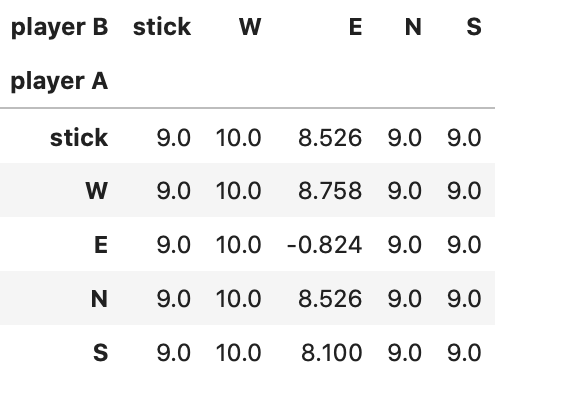
\includegraphics[width=3.4in]{figures/FriendQ_A.png}\\
	(a) player A\\
	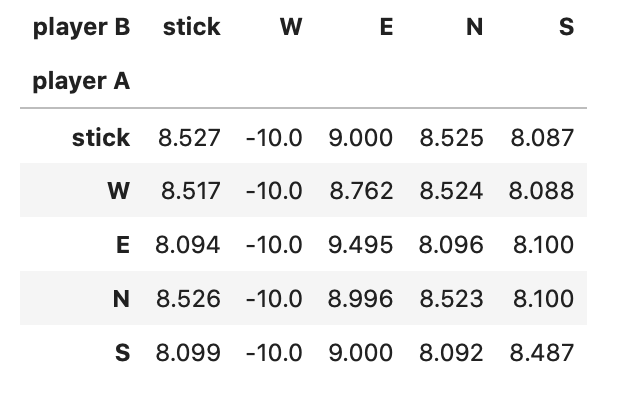
\includegraphics[width=3.4in]{figures/FriendQ_B.png}\\
	(b) player B
	\caption{Q table of state $s$ of trained friend-Q learner}
	\label{fig:friendQ}
\end{figure}

\begin{figure*}
	\begin{tabular}{cc}
		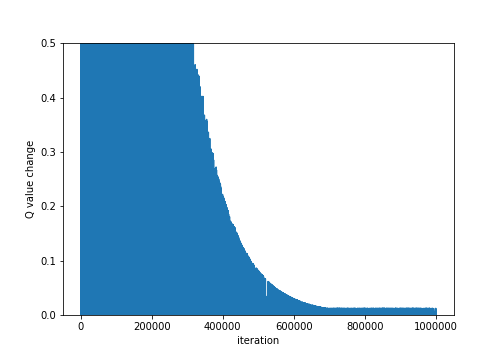
\includegraphics[width=3.4in]{figures/Q.png} &
		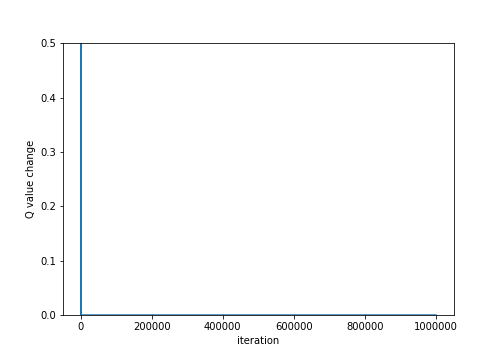
\includegraphics[width=3.4in]{figures/friendQ.png} \\
		(a) Q-Learning & (b) Friend-Q \\
		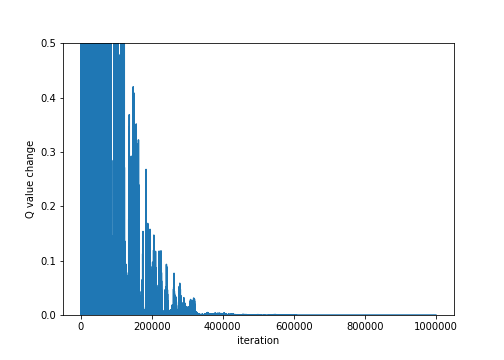
\includegraphics[width=3.4in]{figures/foeQ.png} &
		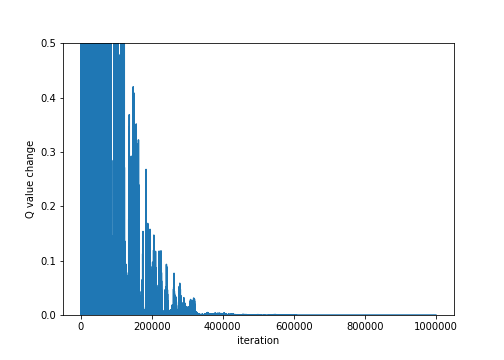
\includegraphics[width=3.4in]{figures/ceQ.png} \\
		(a) Foe-Q & (b) uCE-Q \\
	\end{tabular}
	\caption{}
	\label{fig:results}
\end{figure*}

	
\bibliographystyle{IEEEtran}
\bibliography{reference}

\end{document}
